% 2011 年上海卷（文科）第 20 题：正四棱柱 ABCD-A1B1C1D1（底面边长 1，高 AA1=2）。
% 来源 PDF：普通高考/2011/2011上海文.pdf，SHA-256 ce52f4e95fde8fcfa636f06906fd95c4e685dfbf2bf8e400d8e7cca44a298535。
% 原页：第 1 页（印刷页 699）第 3 栏上部。
% 重绘依据：原图正视略斜视；可见棱为实线，被遮的 AA1、A1B1、A1D1 为虚线；
% 顶点标注 A 在上底后左、D 上底后右、B 上底前左、C 上底前右，A1/D1/B1/C1 对应在下底。
% 比例：高/底边 = 2，与前视方向一致（图中前表面宽 2、高 4）。
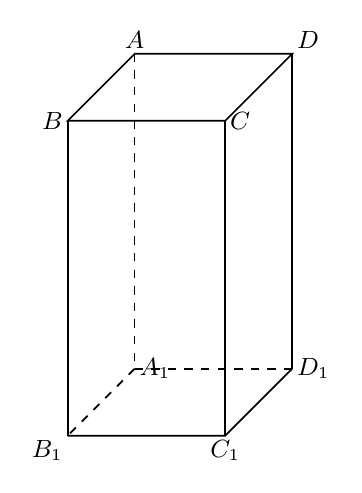
\begin{tikzpicture}[semithick, every node/.style={inner sep=1.5pt, font=\small}]
  \coordinate (B1) at (0,0);
  \coordinate (C1) at (2,0);
  \coordinate (A1) at (0.85,0.85);
  \coordinate (D1) at (2.85,0.85);
  \coordinate (B)  at (0,4);
  \coordinate (C)  at (2,4);
  \coordinate (A)  at (0.85,4.85);
  \coordinate (D)  at (2.85,4.85);
  % 可见棱
  \draw (A) -- (B) -- (C) -- (D) -- cycle;
  \draw (B) -- (B1);
  \draw (C) -- (C1);
  \draw (D) -- (D1);
  \draw (B1) -- (C1) -- (D1);
  % 被遮棱
  \draw[dashed] (A) -- (A1);
  \draw[dashed] (A1) -- (B1);
  \draw[dashed] (A1) -- (D1);
  % 顶点标注
  \node[above] at (A) {$A$};
  \node[above right] at (D) {$D$};
  \node[left] at (B) {$B$};
  \node[right] at (C) {$C$};
  \node[right] at (A1) {$A_1$};
  \node[right] at (D1) {$D_1$};
  \node[below left] at (B1) {$B_1$};
  \node[below] at (C1) {$C_1$};
\end{tikzpicture}
